\documentclass[a4paper,10pt]{article}
\usepackage[utf8]{inputenc}
\usepackage[a4paper,left=1.5cm,right=1.5cm,top=0cm,bottom=1.5cm]{geometry}
\usepackage{parskip}
\usepackage{eurosym}
\usepackage{amsmath}
\usepackage{graphicx}
\usepackage{hyperref}
\usepackage{tikz}
\usepackage{float}
\usepackage{listings}
\usetikzlibrary{positioning}
\usepackage{tikz,pgfplots}
\usepackage{csvsimple}

\title{DM-2583 - Big Data in Media Technology\\Lab 1 - Sentiment Analysis using a Naive Bayes Classifier}
\date{\vspace{-7ex}
Charles \textsc{Hamesse},
Carl \textsc{Holmqvist},
Isak \textsc{Stensö},
Philip \textsc{Stiff}
}
\begin{document}


\maketitle

%
\begin{abstract}
    In this project, we use a dataset containing book reviews to train a natural language classifier for sentiment analysis in further test it on hotel reviews.
    \vspace{2ex}
\end{abstract}
\vspace{-5ex}
%
\section{Process diagram}
\begin{center}
	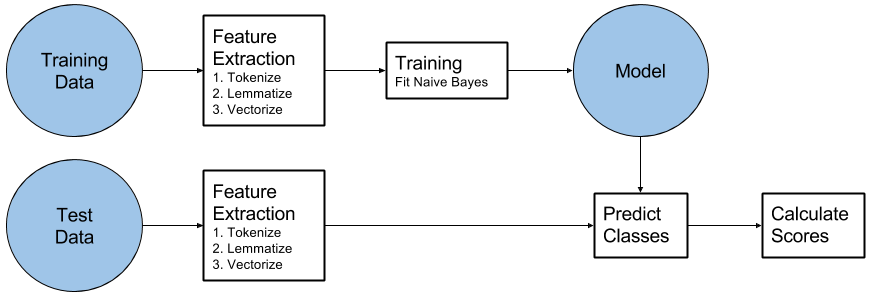
\includegraphics[width=.6\textwidth]{diagram}
\end{center}

%
\section{Feature extraction}
The short texts in the data are tokenized, lemmatized and finally vectorized. By tokenizing the texts we can analyze on individual words. By lemmatizing the words, we get the meaning of the word, and have it in a form so that it can be compared to the same word but inflected differently. By vectorizing them, we turn the text strings into vectors, representing how many time each lemmatized word appears in every string.

Here’s an example of the feature extraction process for the sentence “Brokeback Mountain was really depressing”:
\begin{enumerate}
	\item Tokenize: the sentence becomes a bag of words: Brokeback, Mountain, was, really, depressing
	\item Lemmatize: Brokeback, Mountain, be, really, depress
	\item Vectorize: Term-document matrix representing the frequencies of every dictionary word in the sentence. Brokeback, Mountain, be, really, depress are set to 1, all others are set to 0.
\end{enumerate}

\section{Model implementation}
We used scikit-learn's MultinomialNB model.

\section{Results}
We got 135/200 correct predictions on the test data set using our trained model, representing 67.5\% accuracy. Both the precision and the recall values for the whole data set were roughly 68\%.

\section{Evaluation}
The results are affected by the subjectivity in annotating the test data ourselves. Since different people might annotate the data differently the results will be affected by the annotator. 

68\% is better than randomly guessing, which should (with an unknown test data set) yield 50\% accuracy. However, the results are not overwhelmingly good. One reason could be that the training data is small. Also, the training data contains movie reviews, while the test data contains hotel reviews. It is possible that the different subject matters skew the results. Also, we are analyzing every word independently, regardless of its context. Using bi-grams could potentially yield better results.
	
\end{document}



